\chapter{Implementacija i korisničko sučelje}
		
		
		\section{Korištene tehnologije i alati}
			
			 Komunikacija u timu realizirana je korištenjem aplikacija \underline{WhatsApp}\footnote{https://www.whatsapp.com/} i \underline{Discord}\footnote{https://discord.com/}. Za izradu UML dijagrama korišten je alat \underline{Astah Professional}\footnote{https://astah.net/editions/professional} , a kao sustav za upravljanje izvornim kodom \underline{Git}\footnote{https://git-scm.com/}. Udaljeni repozitorij projekta je dostupan na web platformi \underline{GitLab}\footnote{https://gitlab.com/}.
			 
			 Kao razvojno okruženje korišten je \underline{IntelliJ IDEA}\footnote{https://www.jetbrains.com/idea/} - integrirano razvojno okruženje (IDE) napisano u Javi za razvoj računalnih softvera napisanih u Javi, Kotlinu, Scali, Groovyu i drugim jezicima koji se temelje na JVM-u. Razvio ga je JetBrains (ranije poznat kao IntelliJ) i dostupan je kao Apache 2 licencirano izdanje zajednice (Community Edition) te u vlasničkom komercijalnom izdanju (Ultimate). Oba se mogu koristiti za komercijalni razvoj, a dostupni su za operacijske sustave Windows, macOS i Linux.
			 
			 Aplikacija je napisana koristeći radni okvir \underline{Spring Boot}\footnote{https://start.spring.io/} i jezik \underline{Java}\footnote{https://www.oracle.com/java} za izradu backenda te \underline{React}\footnote{https://reactjs.org/} i jezik \underline{JavaScript}\footnote{https://www.javascript.com/} za izradu frontenda. React, također poznat kao React.js ili ReactJS, je biblioteka u JavaScriptu za izgradnju korisničkih sučelja. Održava je Facebook. React se najčešće koristi kao osnova u razvoju web ili mobilnih aplikacija. Složene aplikacije u Reactu obično zahtijevaju korištenje dodatnih biblioteka za interakciju s API-jem. Spring je radni okvir korišten za olakšan razvoj aplikacija, a omogućava konfiguraciju objekata i lakše upravljanje objektima poslovne logike te općenito brine o kreiranju svih objekata, njihovom povezivanju i čitavom životnom ciklusu. Spring Boot je jedna od komponenti unutar Springa, koja dodatno olakšava njegovo korištenje i omogućava izradu čitavih samostalnih aplikacija. Cilj je ubrzanje i pojednostavljenje razvoja programske potpore.
			 
			 Baza podataka se nalazi na hosting aplikaciji u oblaku, \underline{Render}\footnote{https://render.com/}. Renderova PostgreSQL ponuda olakšava korištenje PostgreSQL-a na siguran, pouzdan i potpuno nesmetan način.\\
			 			
			\eject 
		
	
		\section{Ispitivanje programskog rješenja}
			
			
	
			
			\subsection{Ispitivanje komponenti} 
			
			
			\textbf{1. Testovi za QuizServiceImpl} \\ \\
			Izvorni kod:
				
				\begin{figure}[H]
					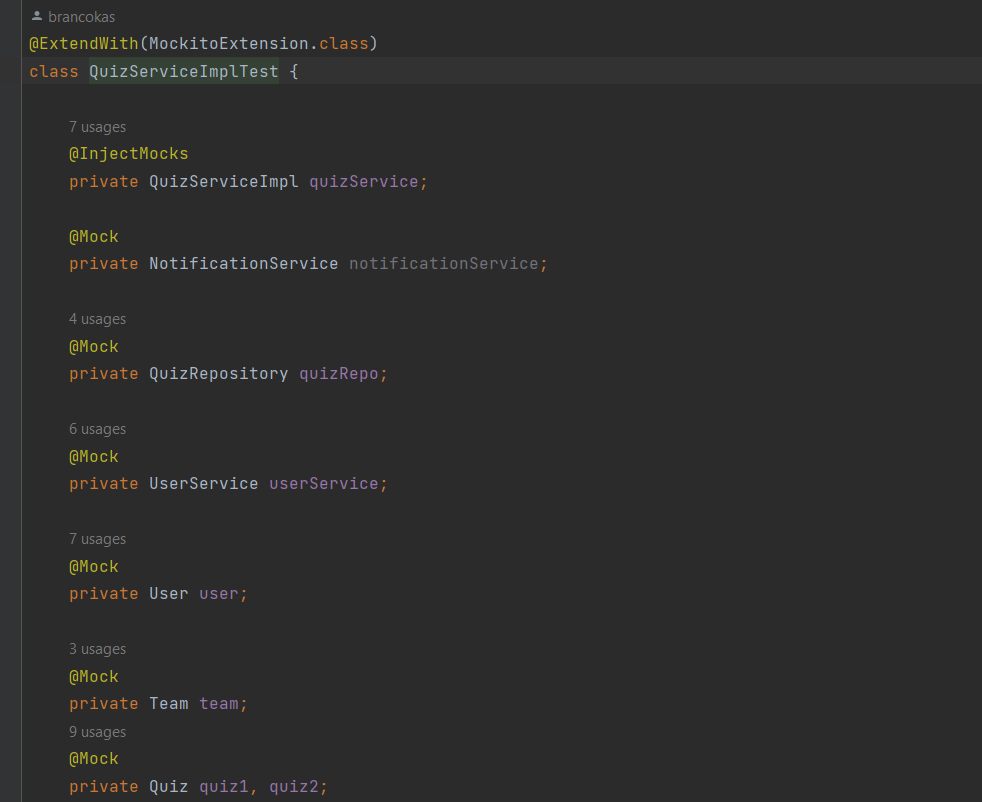
\includegraphics[width=\textwidth]{slike/QuizServiceImplTest1.PNG} 
					\caption{Klasa QuizServiceImplTest}
					\label{fig:QuizServiceImplTest1}
				\end{figure}
			
				\begin{figure}[H]
					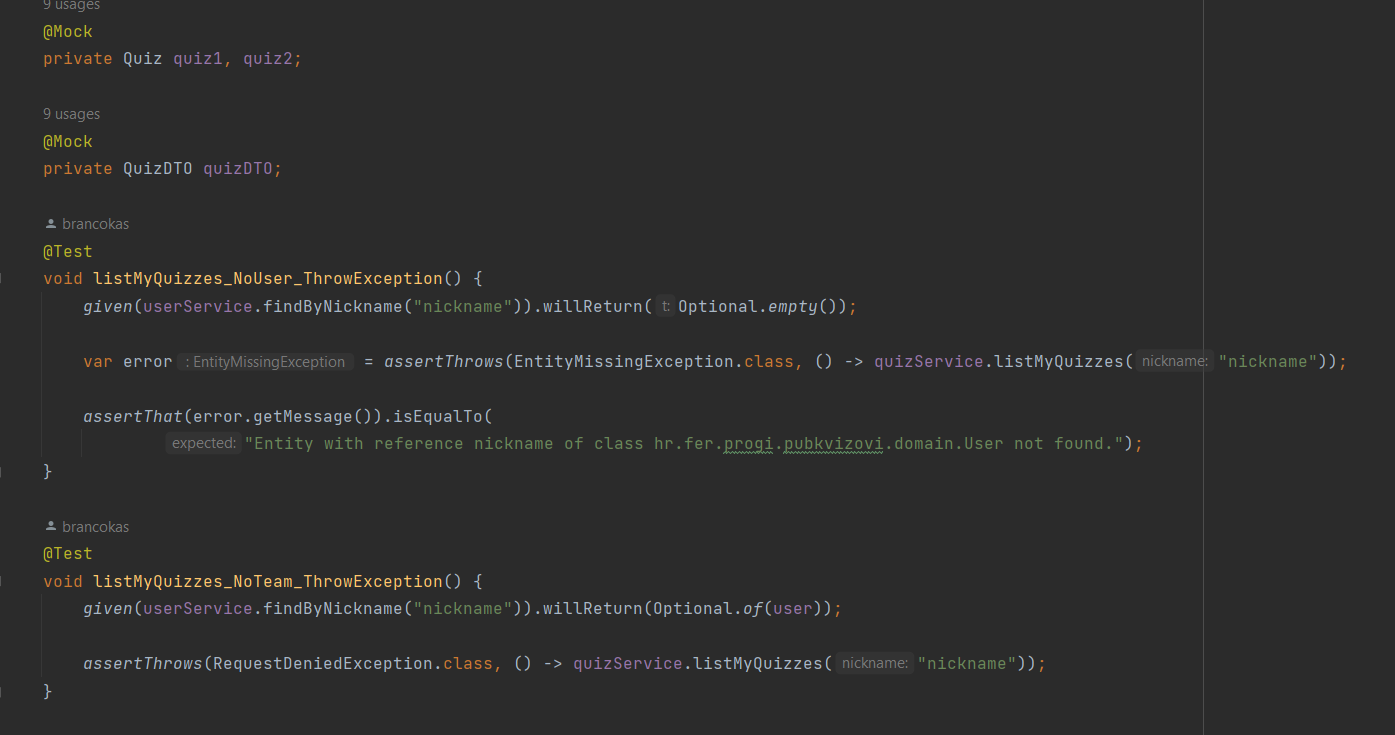
\includegraphics[width=\textwidth]{slike/QuizServiceImplTest2.PNG} 
					\caption{Testovi za listu mojih kvizova, iznimke „nema korisnika” i „nema tima”}
					\label{fig:QuizServiceImplTest2}
				\end{figure}
			
				\begin{figure}[H]
					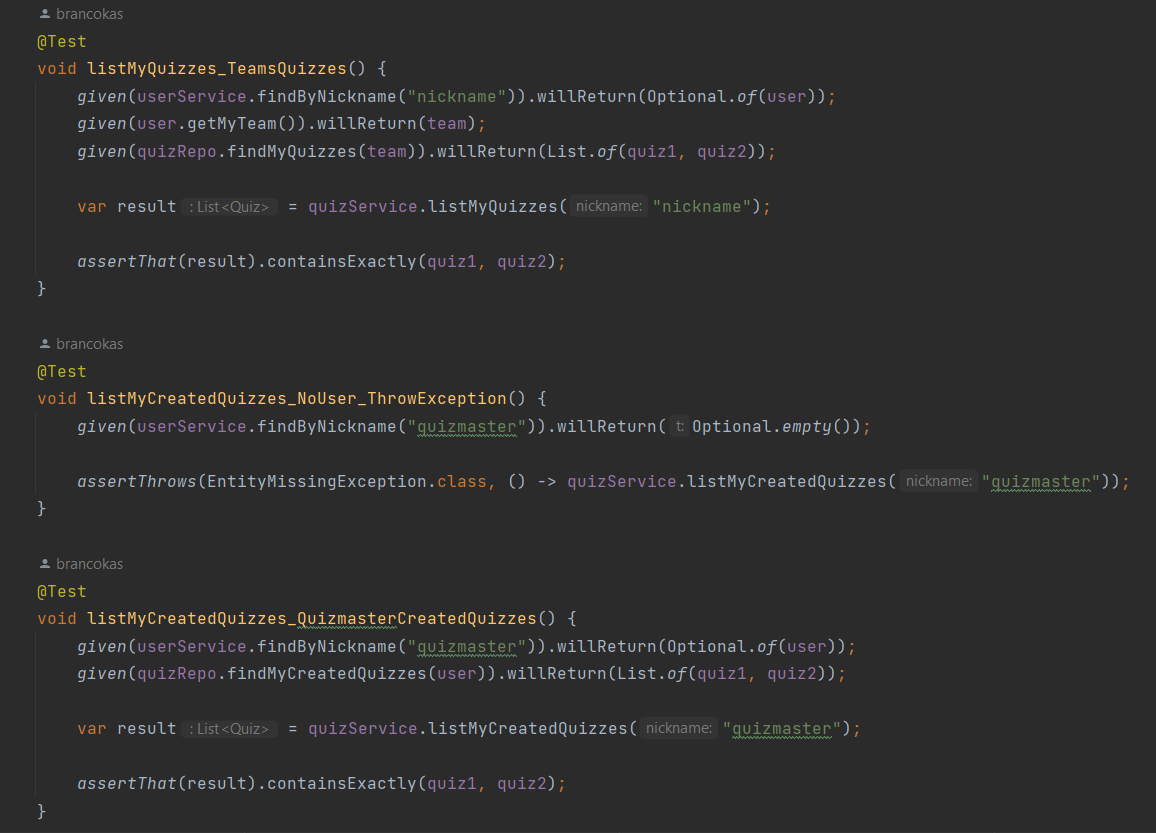
\includegraphics[width=\textwidth]{slike/QuizServiceImplTest3.PNG} 
					\caption{Lista kvizova, iznimka u mojim kreiranim kvizovima „nema korisnika”, lista mojih kreiranih kvizova}
					\label{fig:QuizServiceImplTest3}
				\end{figure}
			
				\begin{figure}[H]
					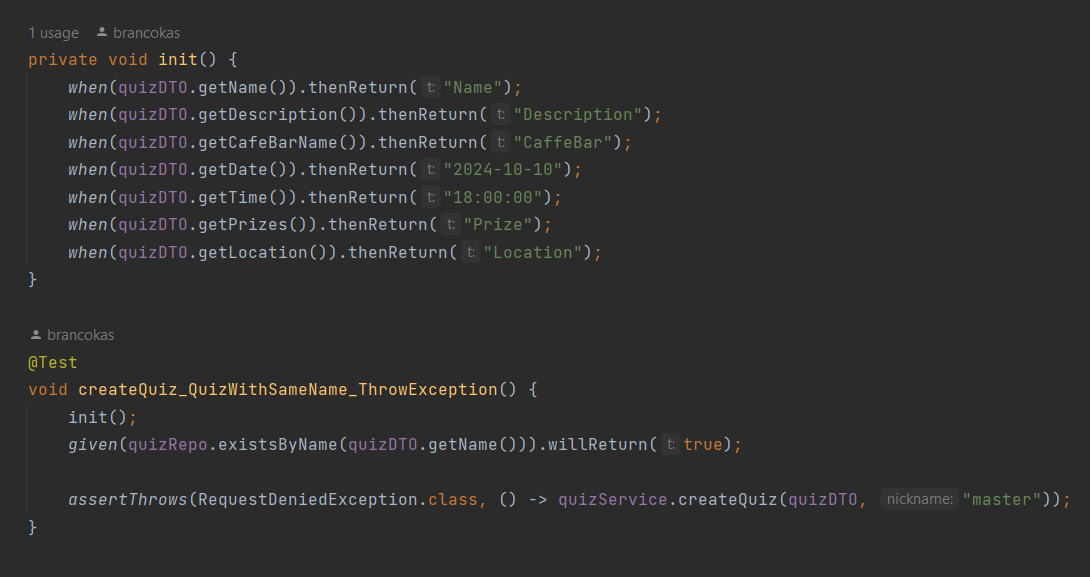
\includegraphics[width=\textwidth]{slike/QuizServiceImplTest4.PNG} 
					\caption{Iznimka, „kreiran kviz sa istim imenom”}
					\label{fig:QuizServiceImplTest4}
				\end{figure}
			
				\begin{figure}[H]
					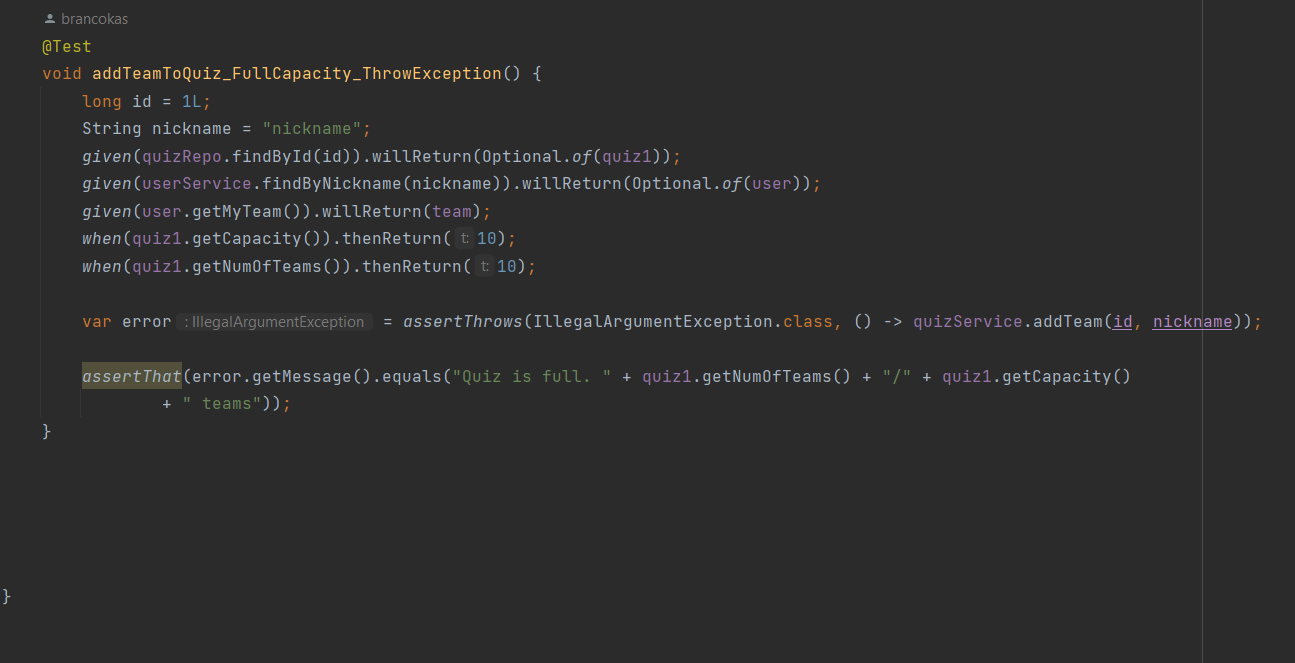
\includegraphics[width=\textwidth]{slike/QuizServiceImplTest5.PNG} 
					\caption{Iznimka za dodavanje tima kvizu, „pun kapacitet”}
					\label{fig:QuizServiceImplTest5}
				\end{figure}
			
				\begin{figure}[H]
					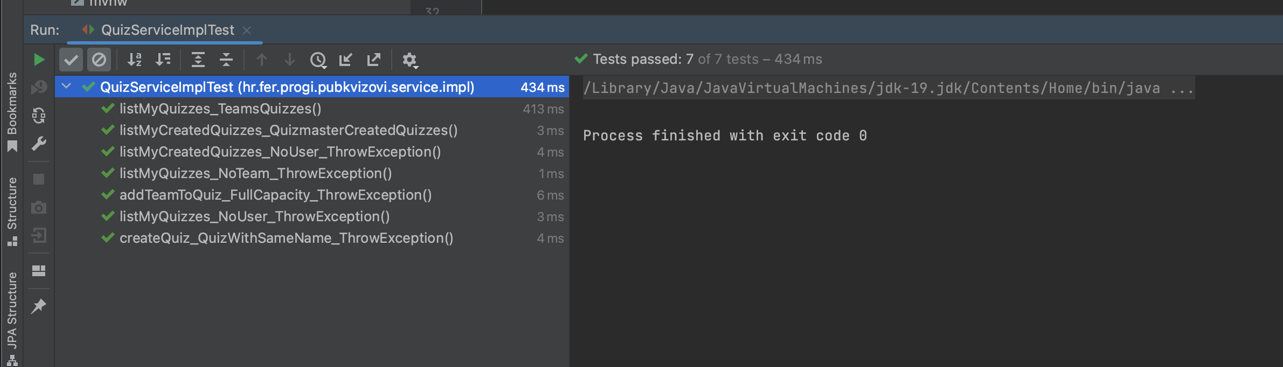
\includegraphics[width=\textwidth]{slike/QuizServiceImplTestRez.PNG} 
					\caption{Rezultati testova}
					\label{fig:QuizServiceImplTestRez}
				\end{figure}
			
			
			
			\textbf{2. Testovi za TeamServiceImpl} \\ \\
			Izvorni kod:
			
				\begin{figure}[H]
					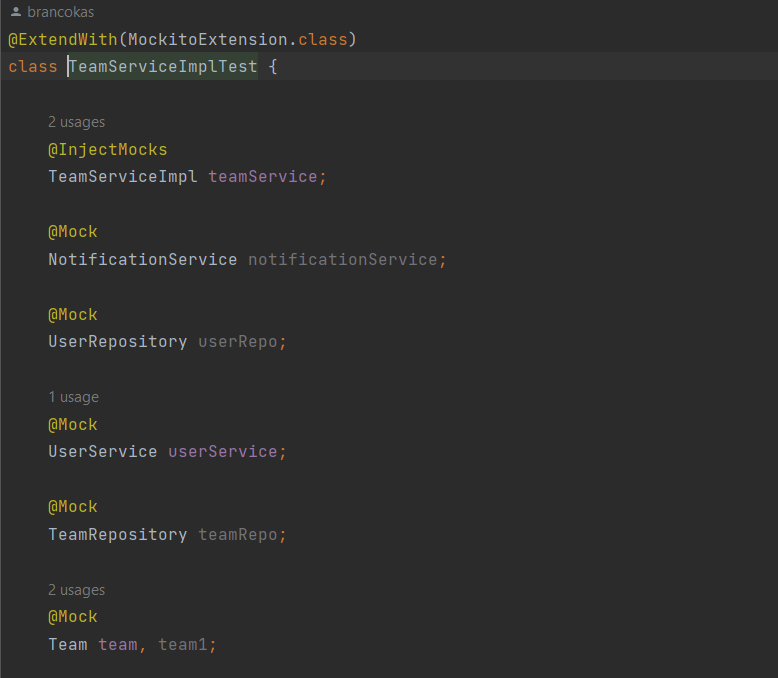
\includegraphics[width=\textwidth]{slike/TeamServiceImplTest1.PNG} 
					\caption{Klasa TeamServiceImplTest}
					\label{fig:TeamServiceImplTest1}
				\end{figure}
			
				\begin{figure}[H]
					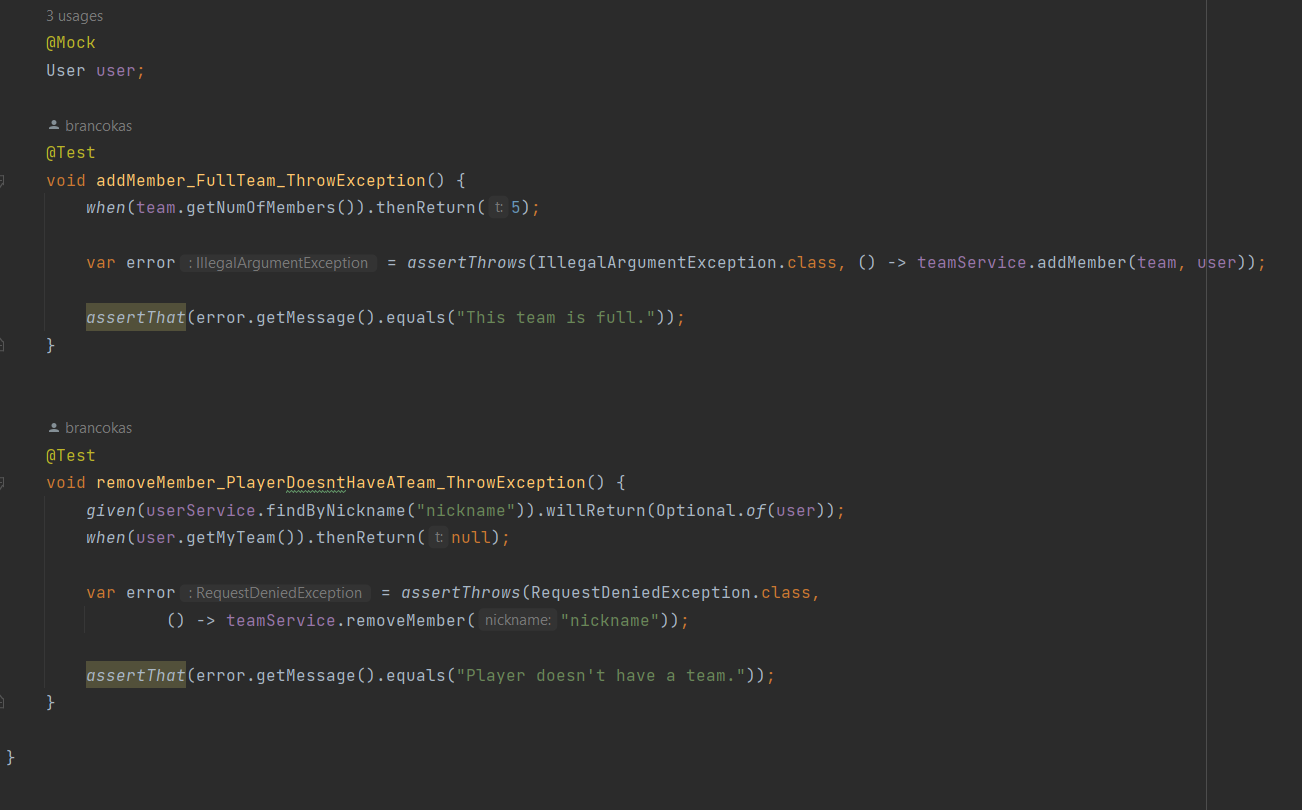
\includegraphics[width=\textwidth]{slike/TeamServiceImplTest2.PNG} 
					\caption{Iznimke, „pun tim” i „igrač nema tim”}
					\label{fig:TeamServiceImplTest2}
				\end{figure}
			
				\begin{figure}[H]
					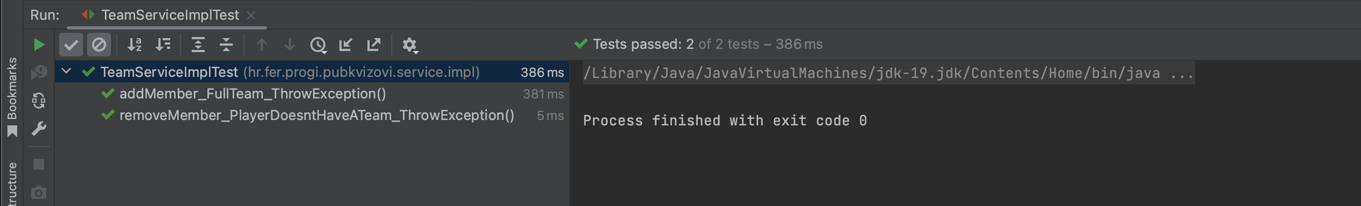
\includegraphics[width=\textwidth]{slike/TeamServiceImplTestRez.PNG} 
					\caption{Rezultati testova}
					\label{fig:TeamServiceImplTestRez}
				\end{figure}
			
			\eject
			
			\textbf{3. Testovi za UserServiceImpl} \\ \\
			Izvorni kod:
				
				\begin{figure}[H]
					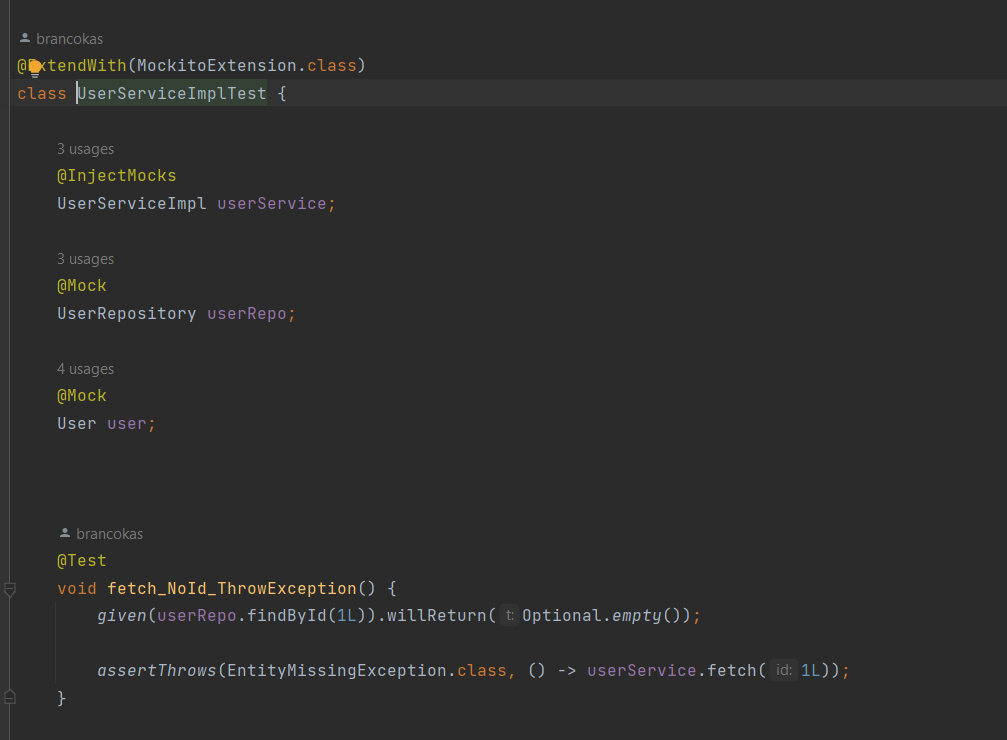
\includegraphics[width=\textwidth]{slike/UserServiceImplTest1.PNG} 
					\caption{Klasa UserServiceImplTest, iznimka „nema id-a”}
					\label{fig:UserServiceImplTest1}
				\end{figure}
				
				\begin{figure}[H]
					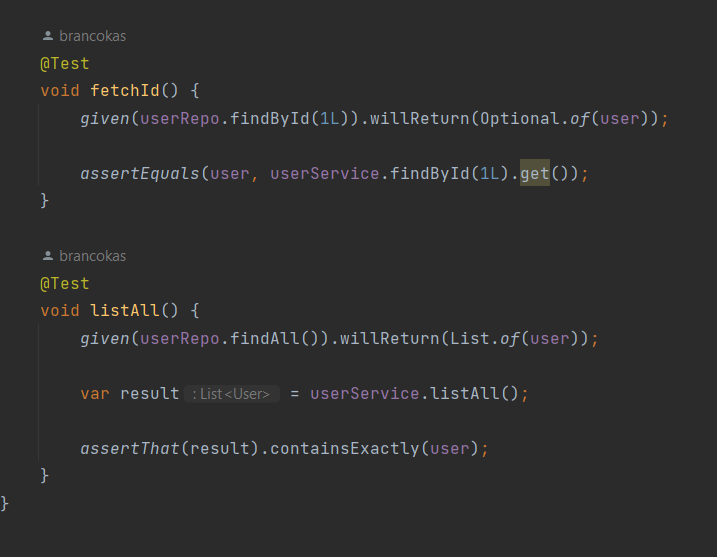
\includegraphics[width=\textwidth]{slike/UserServiceImplTest2.PNG} 
					\caption{Testovi za „dohvati id” i dohvat svih korisnika}
					\label{fig:UserServiceImplTest2}
				\end{figure}
				
				\begin{figure}[H]
					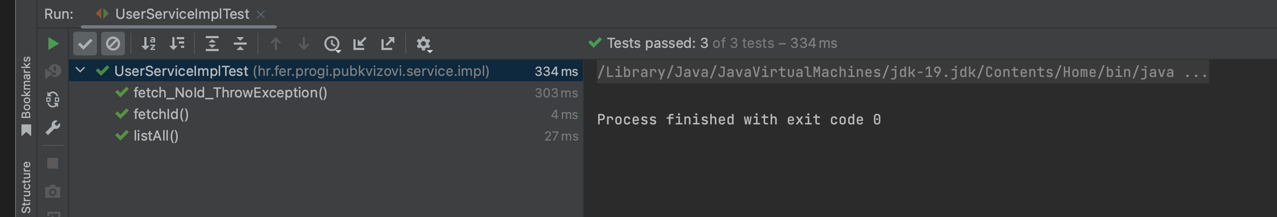
\includegraphics[width=\textwidth]{slike/UserServiceImplTestRez.PNG} 
					\caption{Rezultati testova}
					\label{fig:UserServiceImplTestRez}
				\end{figure}
								
			\eject
			
			\subsection{Ispitivanje sustava}
			 
			\textbf{1. Prijava}\\
				
				Već registrirani korisnik se nalazi na stranici za prijavu. U polja za unos(Nickname i Password) unosi svoje podatke koje je odredio pri registraciji. Ako je prijava uspješna kao u ovom slučaju, prijavljeni korisnik se usmjerava na Home stranicu, odnosno početnu stranicu aplikacije.
				
				\begin{figure}[H]
					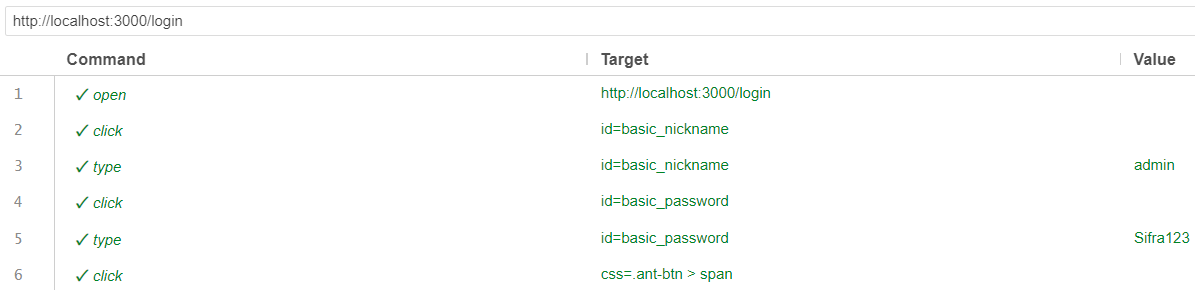
\includegraphics[width=\textwidth]{slike/UspjesnaPrijava1.PNG} 
					\caption{Postavke testa}
					\label{fig:UspjesnaPrijava1}
				\end{figure}

				\begin{figure}[H]
					
\includegraphics[width=\textwidth]{slike/UspjesnaPrijava2.PNG} 
					\caption{Rezultat testa}
					\label{fig:UspjesnaPrijava1}
				\end{figure}
				
			\eject

			\textbf{2. Neuspješna prijava}\\
				
				Korisnik se nalazi na stranici za prijavu te u polja za unos(Nickname i Password) unosi podatke. Nakon unosa i pokušaja prijave, korisniku je javljeno da se nije moguće prijaviti. Sustav mu javlja "You are blocked or your credentials are wrong!". Dvije su mogućnosti zašto se korisnik ne može prijaviti, jedna od njih je ako je korisnik blokiran od strane admina, a druga mogućnost je da je unio krive podatke za prijavu.

				\begin{figure}[H]
					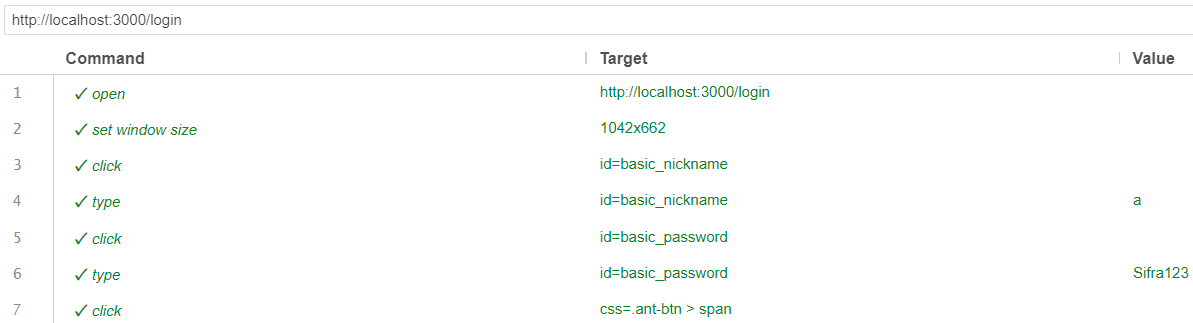
\includegraphics[width=\textwidth]{slike/NeuspjesnaPrijava1.PNG} 
					\caption{Postavke testa}
					\label{fig:NeuspjesnaPrijava1}
				\end{figure}

				\begin{figure}[H]
					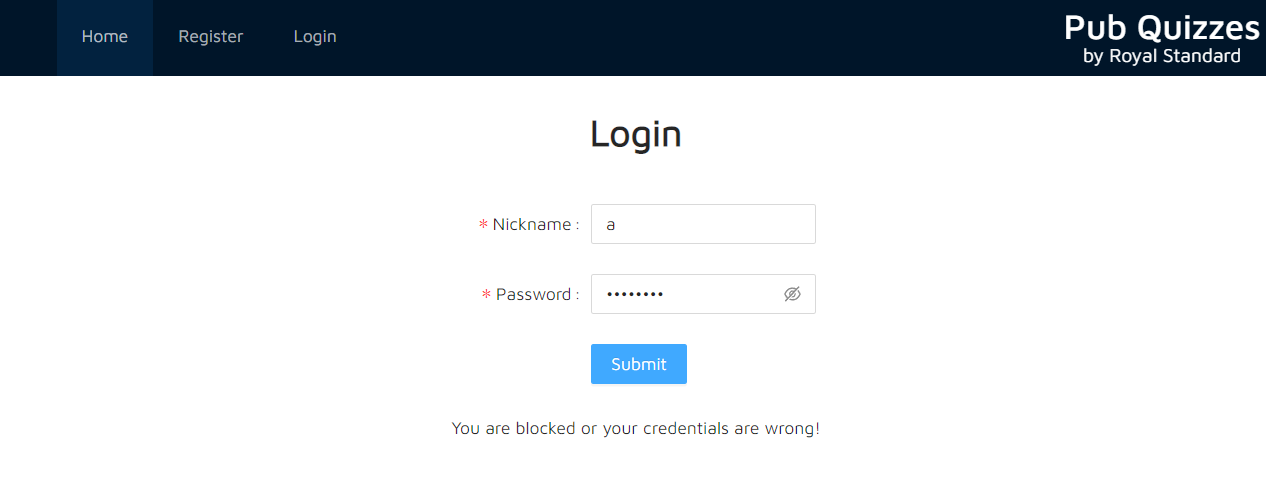
\includegraphics[width=\textwidth]{slike/NeuspjesnaPrijava2.PNG} 
					\caption{Rezultat testa}
					\label{fig:NeuspjesnaPrijava2}
				\end{figure}
				
			\eject

			\textbf{3. Uspješna registracija}\\
				
				Korisnik se nalazi na stranici za registraciju i ispunjava sve potrebne podatke(ime, prezime, nadimak, email, ulogu, područja znanja i šifru). Nakon klika gumba Submit, ako je registracija uspješna kao u ovom slučaju, novoregistrirani korisnik se usmjerava na stranicu za prijavu gdje se s tim istim podatcima mora prijaviti.

				\begin{figure}[H]
					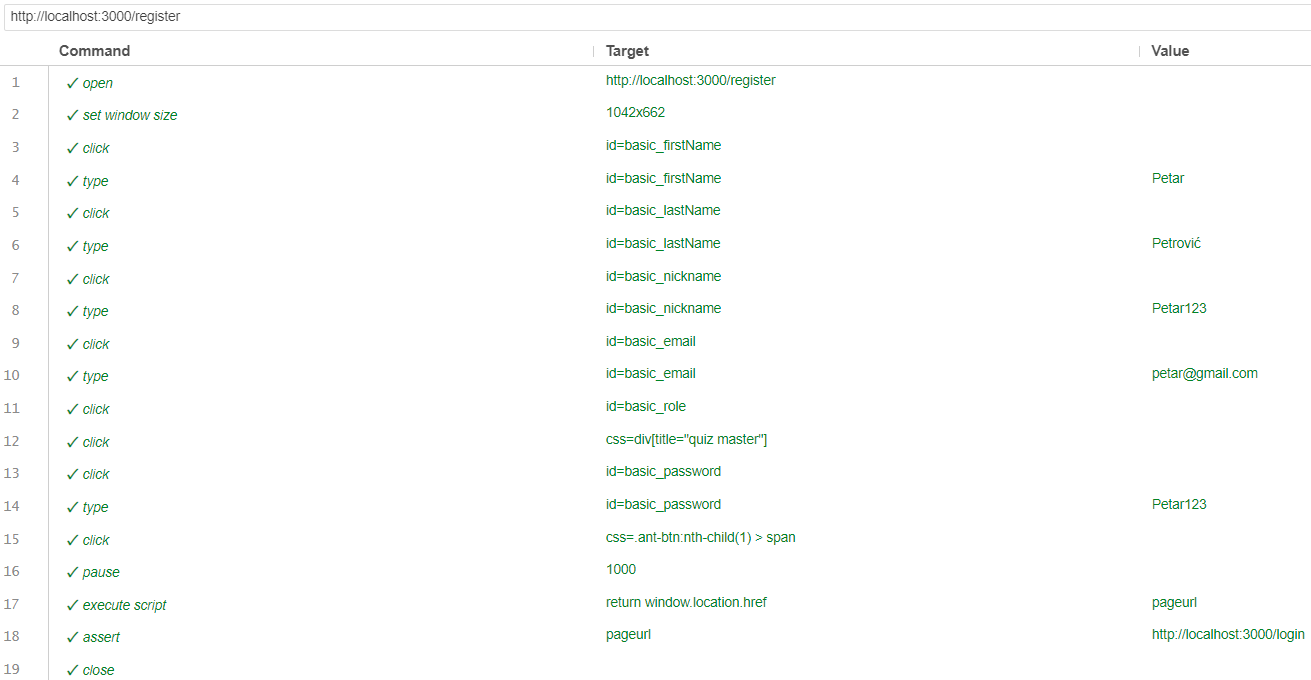
\includegraphics[width=\textwidth]{slike/UspjesnaRegistracija1.PNG} 
					\caption{Postavke testa}
					\label{fig:UspjesnaRegistracija1}
				\end{figure}

				\begin{figure}[H]
					
\includegraphics[width=\textwidth]{slike/UspjesnaRegistracija2.PNG} 
					\caption{Rezultat testa}
					\label{fig:UspjesnaRegistracija2}
				\end{figure}
				
			\eject

			\textbf{4. Neuspješna registracija}\\
				
				Korisnik se nalazi na stranici za registraciju i ispunjava polja, no nije ispunio polja "E-mail" i "Knowledge areas:" koja su obavezna. Nakon klika na gumb Submit, neće doći do uspješne registracije jer korisnik nije unio sve obavezne podatke, pa sukladno tome neće biti registriran.

				\begin{figure}[H]
					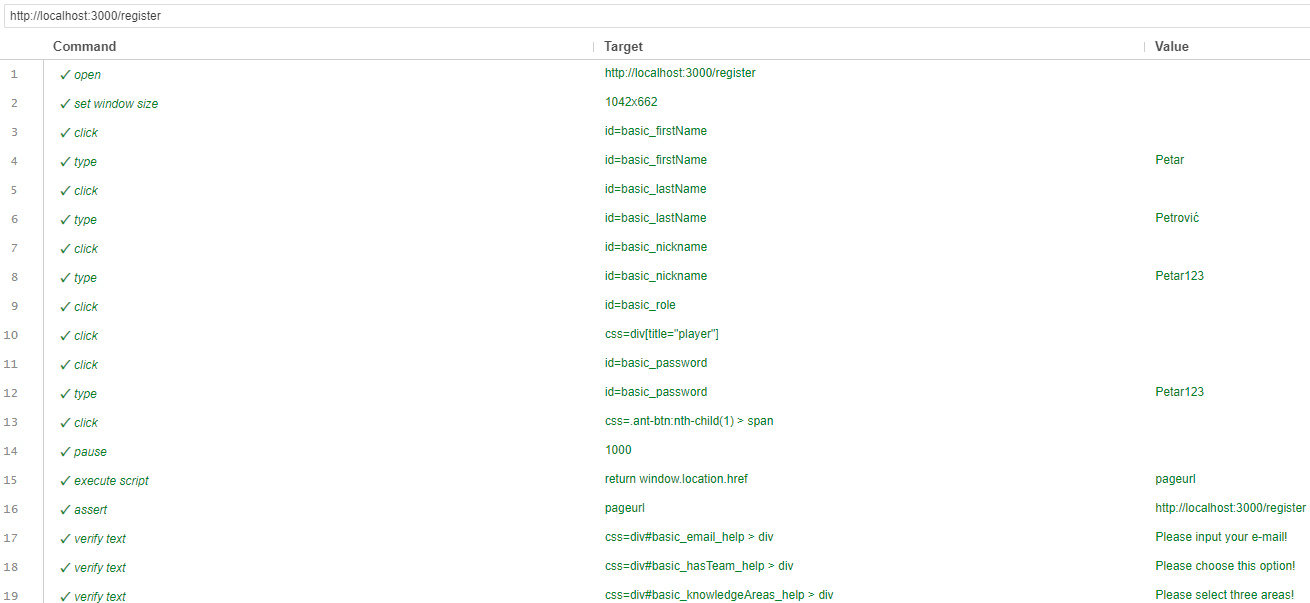
\includegraphics[width=\textwidth]{slike/NeuspjesnaRegistracija1.PNG} 
					\caption{Postavke testa}
					\label{fig:NeuspjesnaRegistracija1}
				\end{figure}

				\begin{figure}[H]
					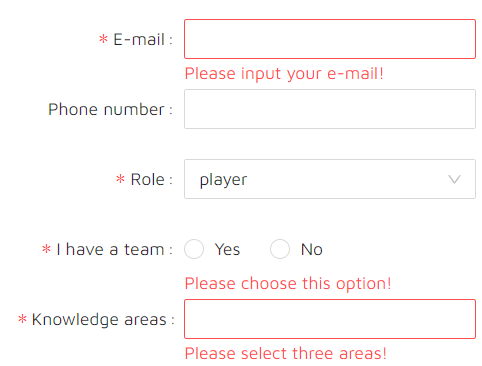
\includegraphics[width=\textwidth]{slike/NeuspjesnaRegistracija2.PNG} 
					\caption{Rezultat testa}
					\label{fig:NeuspjesnaRegistracija2}
				\end{figure}
				
			\eject


		
		
		\section{Dijagram razmještaja}
			
			Dijagram razmještaja je strukturni statički UML dijagram koji opisuje topologiju sustava i općenito je usredotočen na odnos sklopovskih i programskih dijelova. U ovom slučaju klijent se pomoću web preglednika spaja na korisničko sučelje (frontend) preko kojeg komunicira s poslužiteljskom aplikacijom (backend), a za komunikaciju se koristi protokol HTTPS. Korisničko sučelje  implementirano je koristeći radni okviru React.js i pokrenuto je na platformi Render, dok je poslužiteljska aplikacija također pokrenuta na platformi Render, ali ostvarena je pomoću radnog okvira Spring Boot te pokrenuta unutar kontejnera Docker. Baza podataka, u koju backend aplikacija sprema sve podatke, izvodi se na svome poslužitelju, a nalazi se isto na platformi Render.
			
			\begin{figure}[H]
				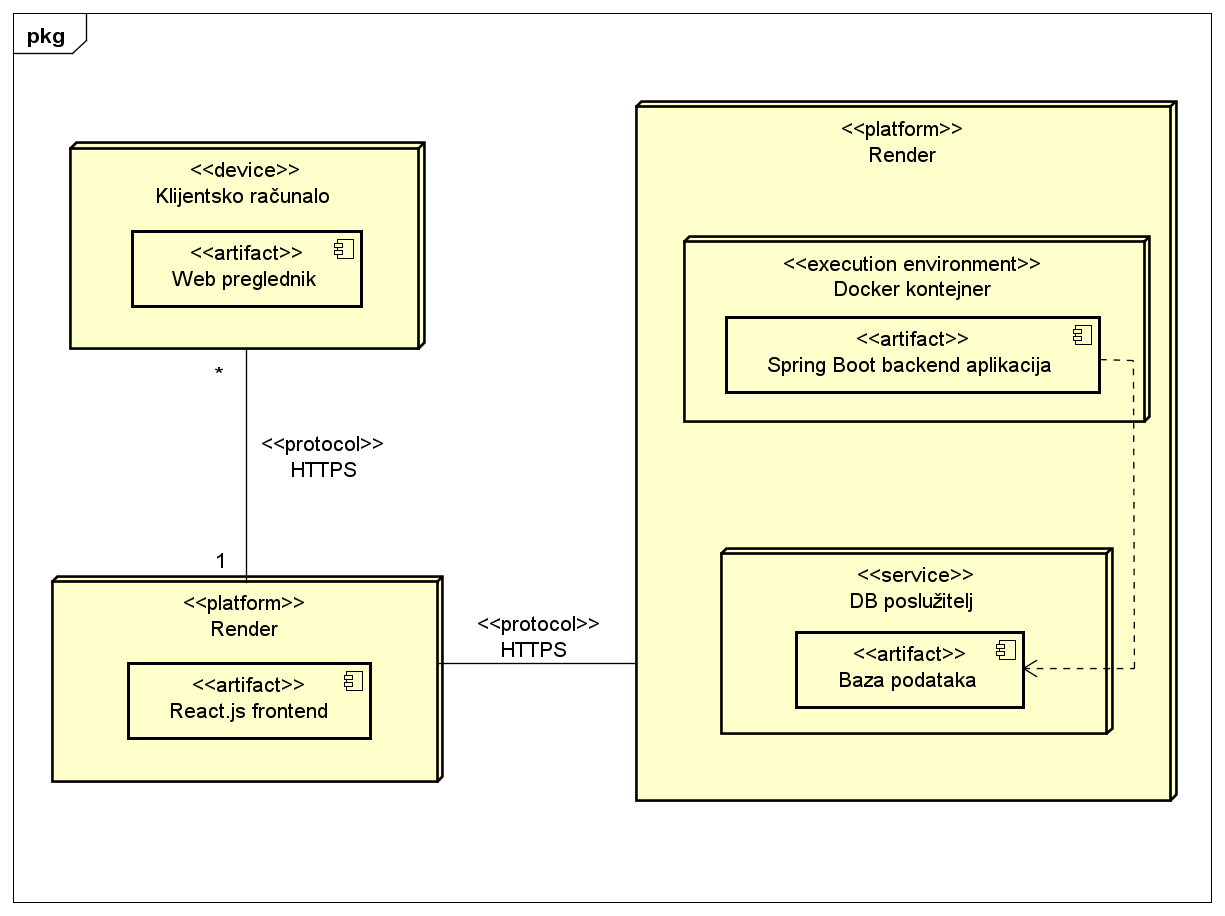
\includegraphics[width=\textwidth]{dijagrami/DeploymentDiagram.PNG} 
				\caption{Dijagram razmještaja}
				\label{fig:DeploymentDiagram}
			\end{figure}
			
			\eject 
		
		\section{Upute za puštanje u pogon}
		
			Za puštanje aplikacije u pogon bila su potrebna tri koraka, odnosno puštanje u pogon svake od tri važne komponente aplikacije, baze podataka, poslužiteljske strane i klijentske strane. To smo radili na platformi Render. 
			
			Izbornik New pokraj korisničkog imena nudi opcije za puštanje u pogon željene komponente aplikacije. U prvom koraku odabrana je opcija „PostgreSQL“ za pohranu baze podataka na platformi. Nakon toga se unesu osnovni podaci o bazi, a platforma Render onda sama generira ostale potrebne podatke (HostName, Password,...). Nakon što je baza postavljena i na platformi, u željenom alatu (odabran PgAdmin) se baza treba registirati pomoću podataka koje je generirala platforma Render i time je puštanje baze podataka u pogon završeno.
			
			\begin{figure}[H]
				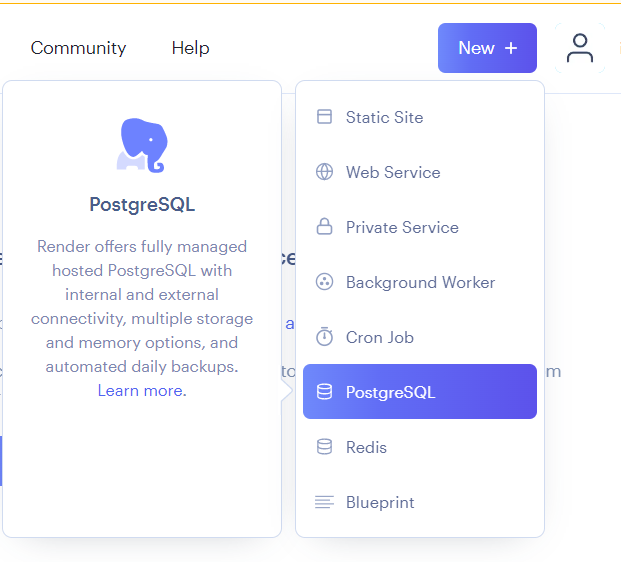
\includegraphics[width=\textwidth]{slike/IzbordnikNew.PNG} 
				\caption{Izbornik za kreiranje novih komponenata}
				\label{fig:Izbornik}
			\end{figure}
		
		\begin{figure}[H]
			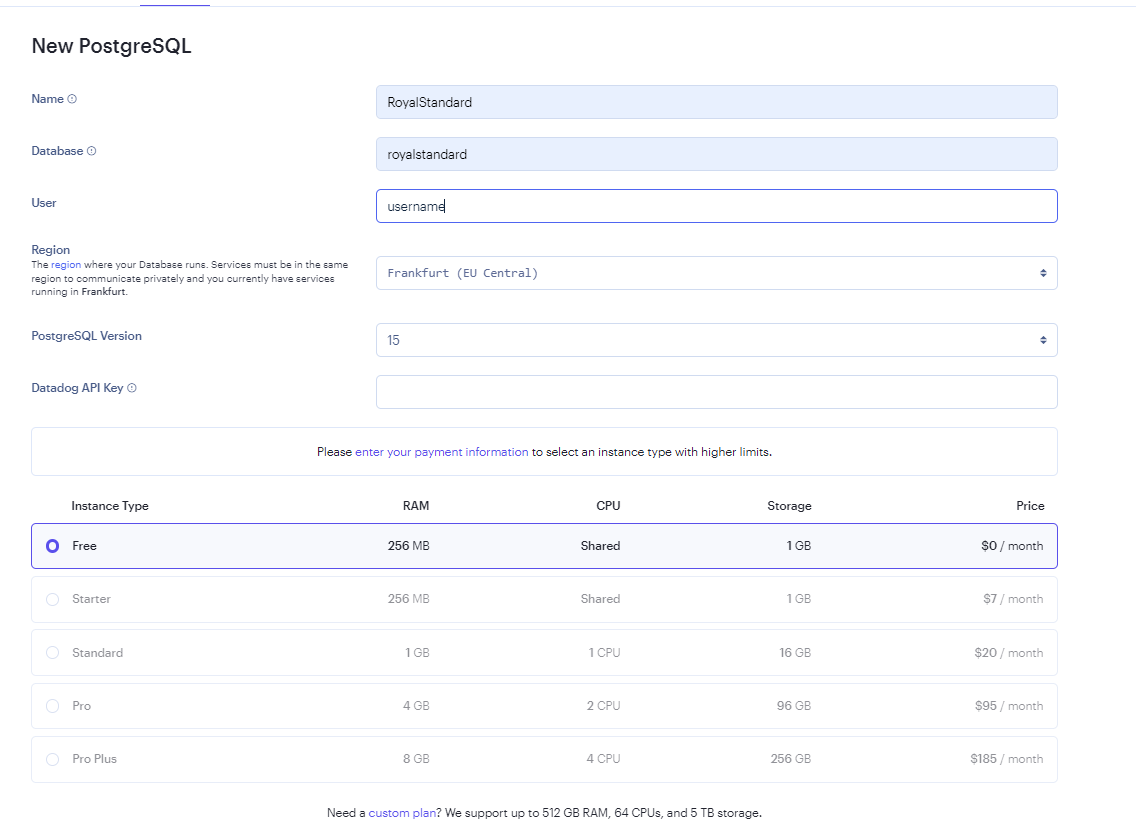
\includegraphics[width=\textwidth]{slike/OsnovniPodaciBaza.PNG} 
			\caption{Upisivanje početnih podataka za bazu podataka}
			\label{fig:Početni podaci za bazu podataka}
		\end{figure}
		
		\begin{figure}[H]
			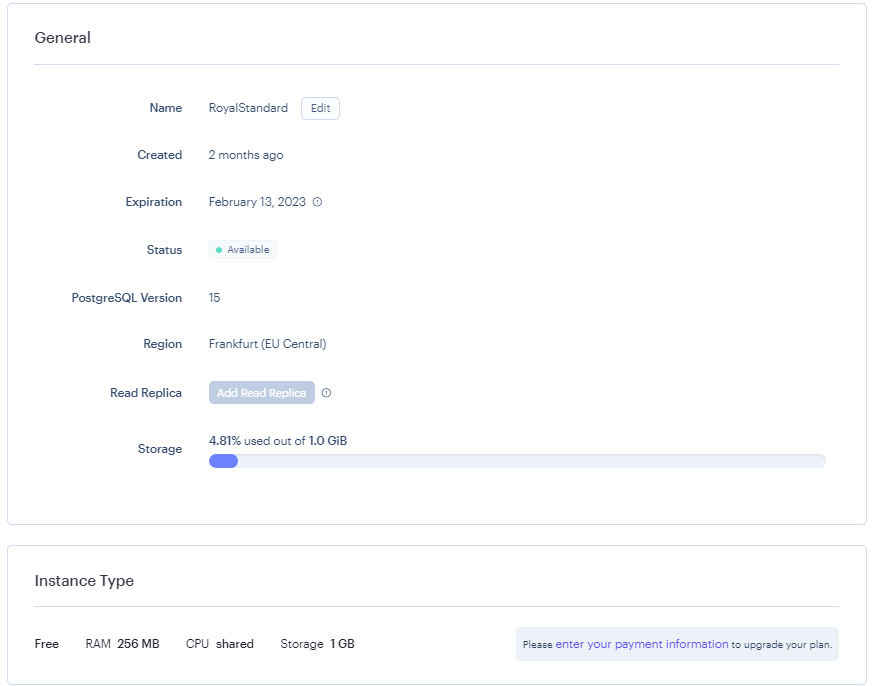
\includegraphics[width=\textwidth]{slike/Baza1.PNG} 
			\caption{Generirani podaci za bazu podataka}
			\label{fig:Generirani podaci za bazu}
		\end{figure}
		
		\begin{figure}[H]
			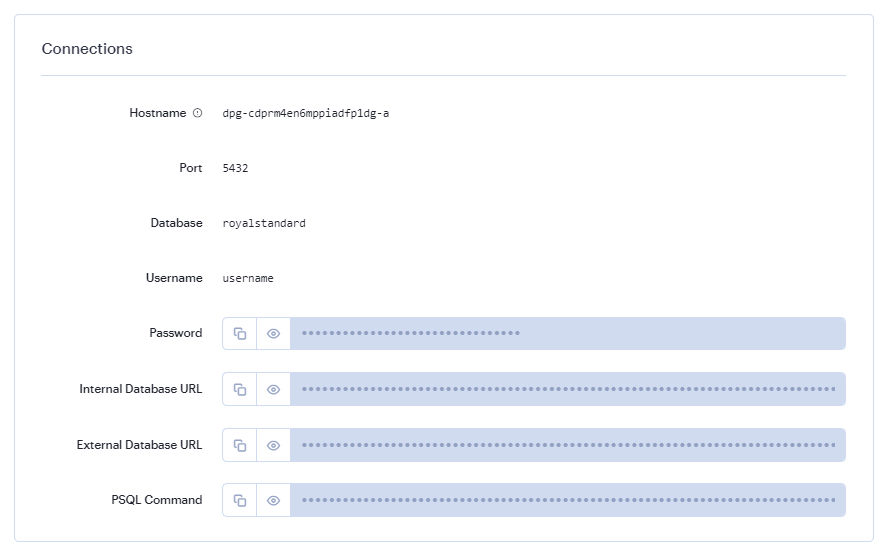
\includegraphics[width=\textwidth]{slike/Baza2.PNG} 
			\caption{Generirani podaci za bazu podataka}
			\label{fig:Generirani podaci za bazu}
		\end{figure}
	
		\begin{figure}[H]
			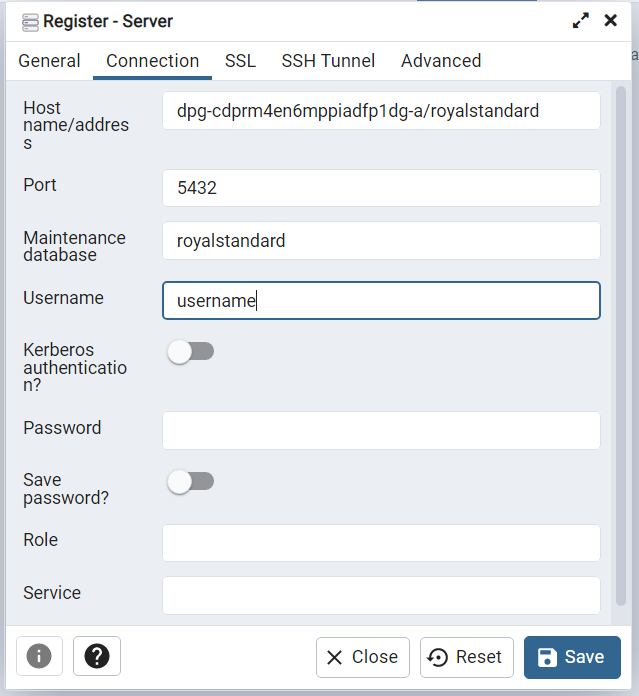
\includegraphics[width=\textwidth]{slike/registracijaservera.PNG} 
			\caption{Registracija servera u sučelju PgAdmin alata}
			\label{fig:Registracija servera baze podataka}
		\end{figure}
	
		
		Za puštanje u pogon poslužiteljske strane u izborniku New platforme Render odabire se opcija WebService te se ostvaruje veza s GitLab repoziorijem iz kojeg se dohvaća kod. Svaki put kad dođe do promjene u repozitoriju, puštanje u pogon će se obaviti automatski ponovno. Osim ispunjavanja osnovnih podataka o poslužiteljskoj strani na Renderu, potrebno je i u kodu unijeti određene promjene. Osim Dockerfile-a, treba ažurirati i datoteku application.properties s podacima za povezivanje s bazom podataka. 
		
		\begin{figure}[H]
			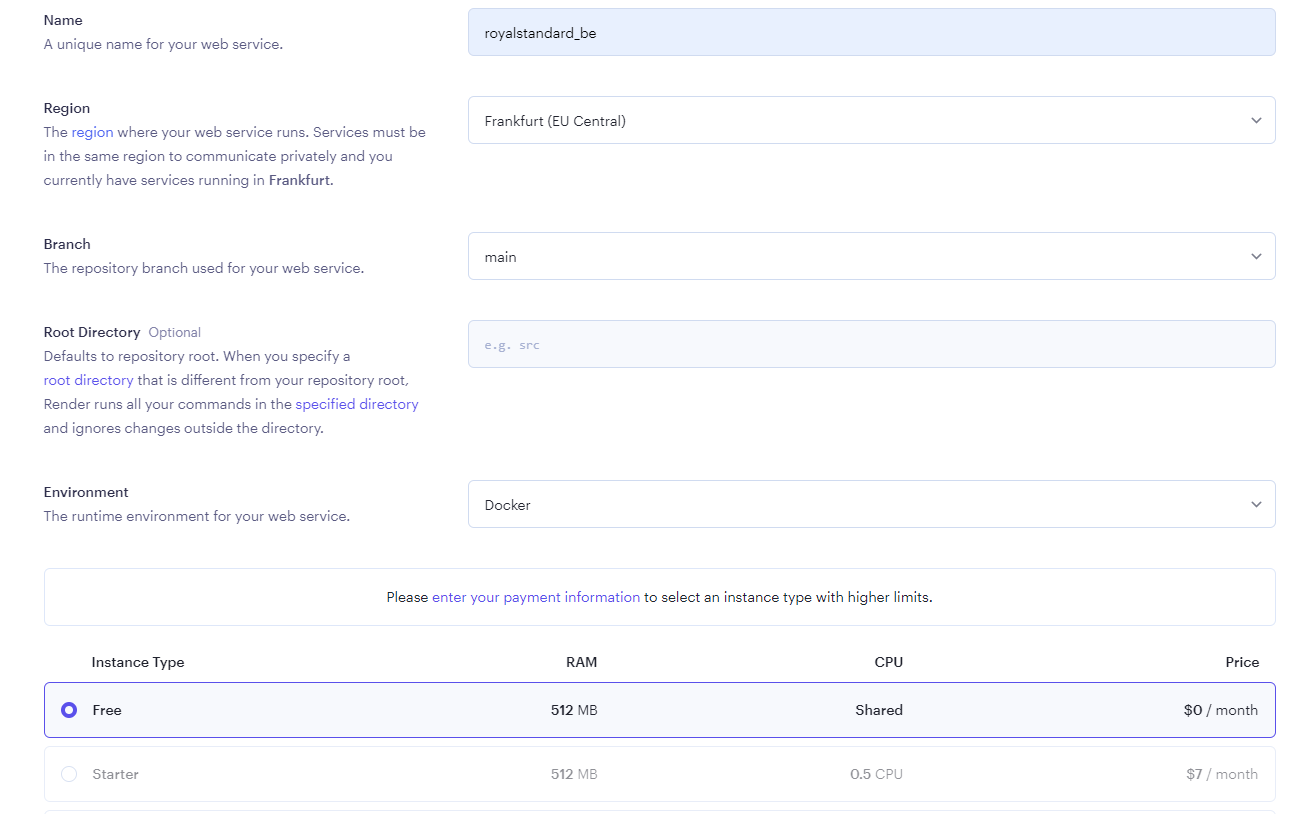
\includegraphics[width=\textwidth]{slike/osnovnipodacibackend.PNG} 
			\caption{Podaci za poslužiteljsku stranu}
			\label{fig:Podaci za poslužiteljsku stranu}
		\end{figure}
	
		\begin{figure}[H]
			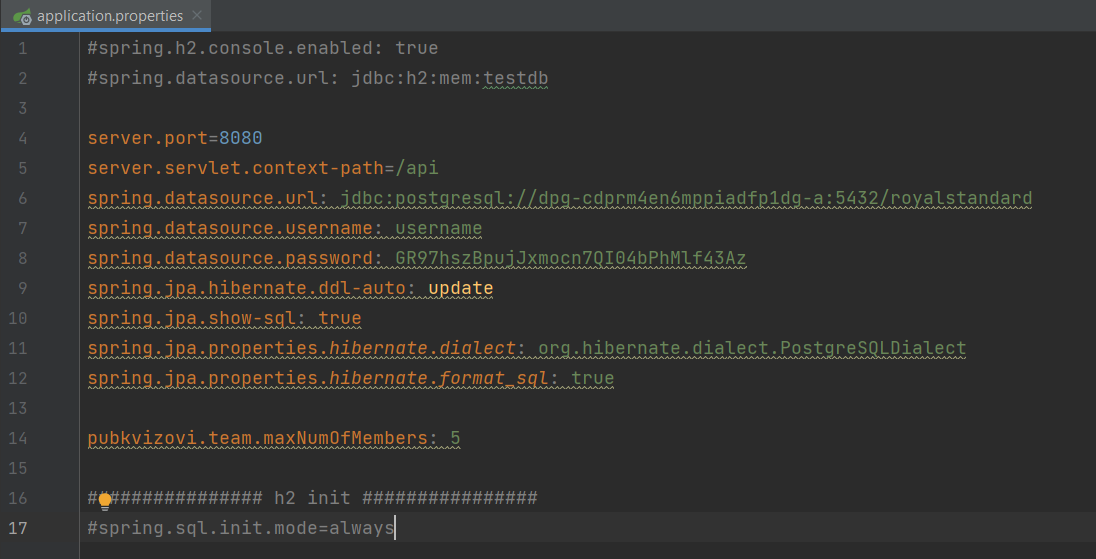
\includegraphics[width=\textwidth]{slike/applicationproperties.PNG} 
			\caption{Datoteka "application.properties"}
			\label{fig:application.properties}
		\end{figure}
		
		\begin{figure}[H]
			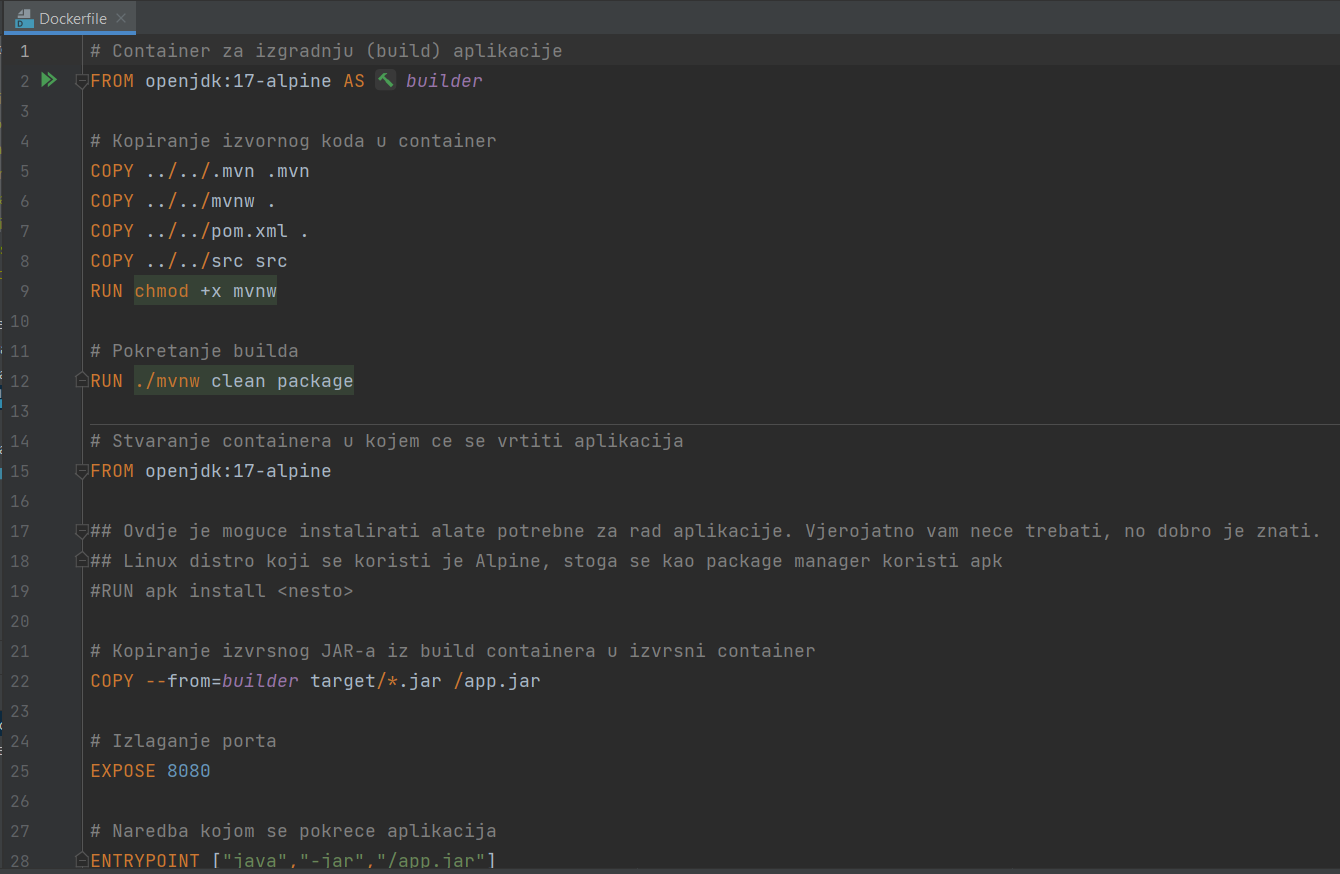
\includegraphics[width=\textwidth]{slike/dockerfile.PNG} 
			\caption{Datoteka "Dockerfile"}
			\label{fig:Dockerfile}
		\end{figure}
		
		Za puštanje u pogon klijentske strane odabire se opcija „WebService“ kao i u prethodnom koraku, ali se upisuju drugačiji podaci (npr. Environment je sada Node i postavljaju se „build command“ kao i „start command“). U environment varijable dodaje se varijabla API-BASE-URL koja se postavlja na adresu poslužiteljske strane. U kodu se kreira datoteka „setupProxy.js“ u kojoj se zahtjevi preusmjeravaju na poslužiteljsku stranu.
			
		
		\begin{figure}[H]
			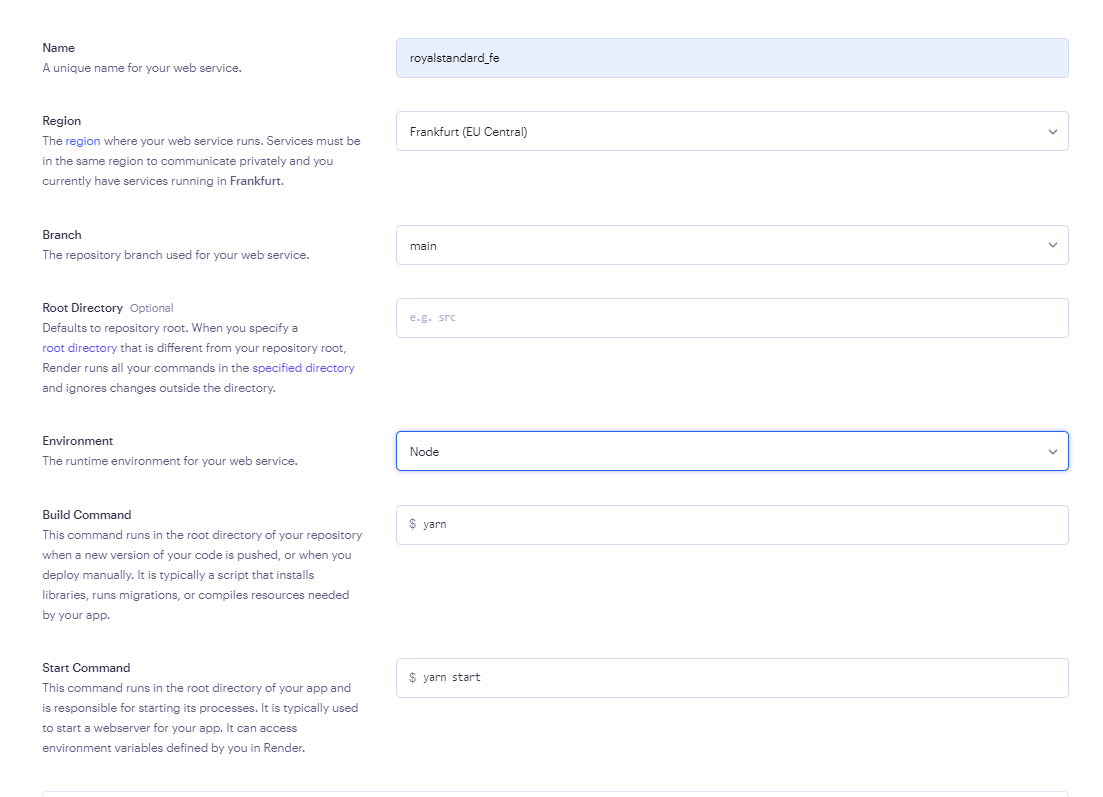
\includegraphics[width=\textwidth]{slike/osnovnipodacifrontend.PNG} 
			\caption{Podaci za klijentsku stranu}
			\label{fig:Podaci za klijentsku stranu}
		\end{figure}
		
		\begin{figure}[H]
			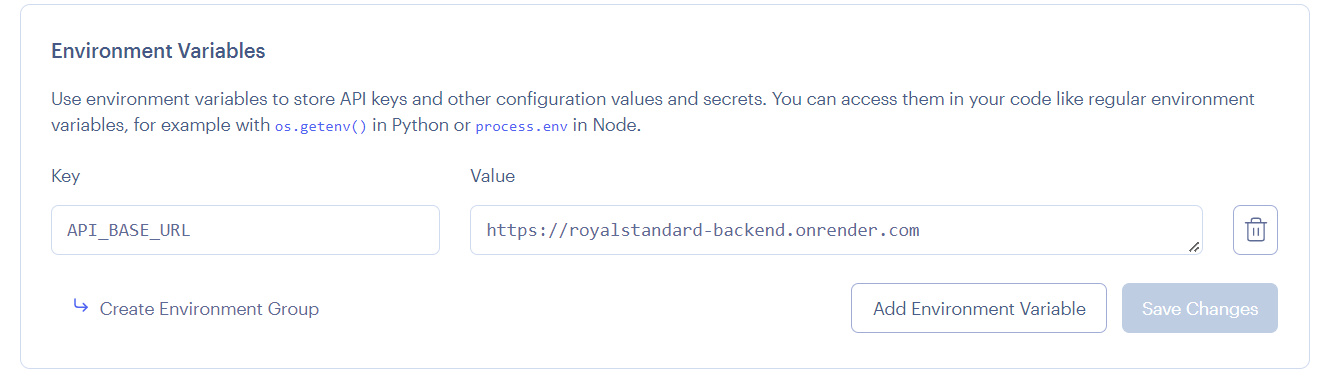
\includegraphics[width=\textwidth]{slike/environmentbaseurl.PNG} 
			\caption{Postavljanje varijable okruženja API-BASE-URL}
			\label{fig:Varijabla okruženja}
		\end{figure}	
	
	\begin{figure}[H]
		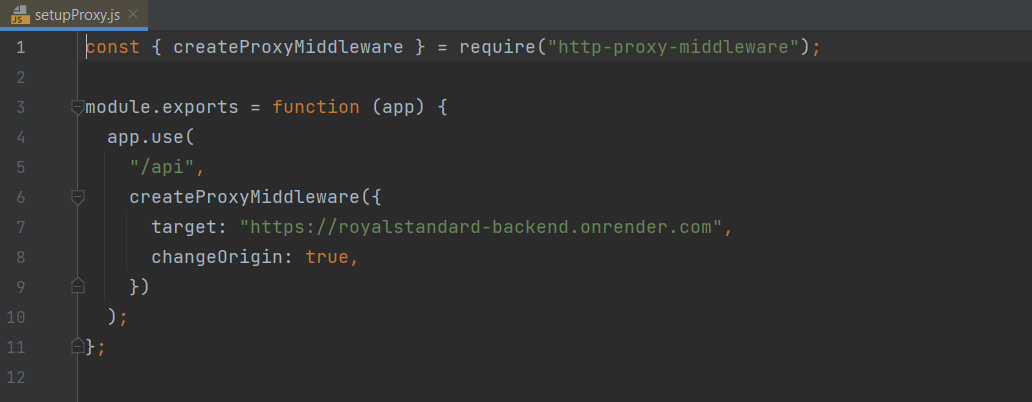
\includegraphics[width=\textwidth]{slike/setupproxy.PNG} 
		\caption{Datoteka "setupProxy.js"}
		\label{fig:Proxy}
	\end{figure}	
			\eject 